\documentclass[12pt]{article}

\usepackage[margin=1in]{geometry}
\usepackage{graphicx}
\graphicspath{{images/}}
\usepackage{subfiles}

\title{\huge Examen de statistique multidimensionnelle}
\author{Groupe 8 :\\
HUYLENBROECK Florent\\
BOSSART Laurent}
\date{Juin 2020}

\begin{document}
\maketitle
\newpage
\tableofcontents
\newpage
\section{Introduction}
Dans le cadre de notre cours de statistique multidimensionnelle il nous a été demandé de, sur base d'un fichier de donnée nommé \emph{XXData}.
\begin{itemize}
\item Effectuer une analyse univariée des données.
\item Effectuer une ACP et en discuter les résultats.
\item Effectuer une classification des individus et des variables et en discuter les résultats.
\end{itemize}
Pour cela, nous allons utiliser le langage de programmation \emph{R} via l'outil \emph{RStudio}.\\
Il nous a aussi été demandé de présenter une technique d'analyse multivariée non vue en cours : \emph{CLARA} (Clustering Large Applications) et d'en décrire un exemple en R.
\section{Analyse univariée des données}
Pour commencer l'analyse de nos données, commencons par jeter un oeil au fichier de donnée en utilisant la fonction \emph{head} de R.
\begin{figure}[h]
\centering
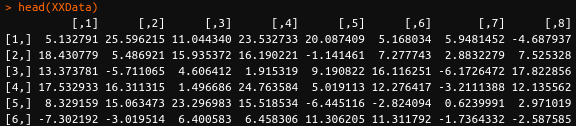
\includegraphics[scale=.75]{head.png}
\caption{Appel et résultat de la fonction head sur XXData}
\end{figure}
\section{ACP}
\section{Classification}
\section{CLARA}
\subfile{CLARA}
\section{Conclusion}

\end{document}
